\documentclass[../notes.tex]{subfiles}

\pagestyle{main}
\renewcommand{\chaptermark}[1]{\markboth{\chaptername\ \thechapter\ (#1)}{}}
\setcounter{chapter}{7}

\begin{document}




\chapter{Mossbauer and EChem}
\section{Mossbauer Spectroscopy}
\begin{itemize}
    \item \marginnote{2/21:}HW will be posted tonight. Due on 3/2.
    \item Final is still on the same date.
    \item Mossbauer is pretty short, so we may start on NMR today, too. NMR will be at least 2 lectures.
    \item Mossbauer was discovered by Rudolf Mossbauer in 1958 when he was 29. He won the Nobel for it in 1961 at age 32.
    \item Basic principle: Involves the resonant nuclear absorption of a gamma rays.
    \begin{itemize}
        \item We use these rays to excite spin flips.
    \end{itemize}
    \item Generating gamma rays: A source nuclei \ce{A} in an excited state decays, emitting a gamma ray with energy $E_\gamma$ which will excite our resonant absorption nucleus \ce{B} and raise it up in energy by $E_r$.
    \item Common source nuclei to use.
    \begin{table}[h!]
        \centering
        \small
        \renewcommand{\arraystretch}{1.2}
        \begin{tabular}{ccccc}
            \textbf{Common Nuclei} & \textbf{$\bm{E_\gamma}$ (keV)} & \textbf{Precursor Nucleus} & \textbf{$\bm{T_{1/2}}$} & \textbf{Abundance}\\
            \hline
            \ce{{}^57Fe} & 14.4 & \ce{{}^57Co} & \SI{267}{\day} & 2.2\%\\
            \ce{{}^124I} & 26.8 & \ce{{}^125Te} & \SI{33}{\day} & 0.63\%\\
            \ce{{}^119Sn} & 23.9 & \ce{{}^{119m}Sn} & \SI{245}{\day} & 8.6\%\\
            \ce{{}^195Pt} & 99 & \ce{{}^195Au} & \SI{192}{\day} & 33.8\%\\
            \ce{{}^61Ni} & 67.4 & \ce{{}^61Co} & \SI{1.65}{\hour} & 1.2\%\\
        \end{tabular}
        \caption{Typical Mossbauer gamma ray source nuclei.}
        \label{tab:MossbauerSources}
    \end{table}
    \begin{itemize}
        \item 90\% or more of Mossbauer is done with \ce{{}^57Fe}.
        \begin{itemize}
            \item At \SI{14.4}{\kilo\electronvolt}, it's a pretty hot but not super hot $\gamma$ ray.
            \item The cobalt precursor nucleus comes from Russia, so a lot of Mossbauer spectroscopists are probably looking at very lean times right now.
        \end{itemize}
        \item \ce{{}^119Sn} is also pretty common.
        \begin{itemize}
            \item With respect to the precursor nucleus, 119m means a \textbf{metastable} state of tin.
        \end{itemize}
    \end{itemize}
    \item There are a few synchrotrons in the world that are set up to do Mossbauer as well. Argonne is one of them! Even with a synchrotron source, though, not all nuclei are good; you need a long-ish life time, or your peak is just gonna be way too broad.
    \item The most common equation in Mossbauer.
    \begin{equation*}
        E_\gamma = E_R+D-R
    \end{equation*}
    \begin{itemize}
        \item $R$ is the recoil energy.
        \begin{itemize}
            \item Gamma rays are so powerful that when one is emitted, there is literally a shotgun-style recoil of the emitting nucleus.
            \item If you lose too much energy to recoil KE, your gamma rays may not match the target source.
            \item Thus, you try to hold your atoms very stable, usually by embedding them in a solid lattice.
        \end{itemize}
        \item $D$ is the doppler energy.
        \begin{itemize}
            \item A Doppler shift is relevant to the experimental setup of Mossbauer.
            \item Essentially, you literally hook up your emitter to a speaker and vibrate it at a hertz frequency to add or subtract a tiny bit of energy to/from the gamma rays.
            \item This setup allows you to get resolution in a very small window around a certain excitation energy of your nucleus.
            \item It also leads to the common unit of \si[per-mode=symbol]{\milli\meter\per\second}.
        \end{itemize}
    \end{itemize}
    \item \textbf{Recoil free fraction}: The fraction of atoms of the source material that are held still enough that $R$ is minimized.
    \item Mossbauer is one of the only techniques that provides direct information about nuclei.
    \item Three main factors that influence the energy of a Mossbauer transition (i.e., quantities you can pull out of the data).
    \begin{enumerate}
        \item Electron density at the nucleus.
        \begin{itemize}
            \item Usually measured by the \textbf{isomer shift} $\delta$ (think \si{\ppm} from NMR).
            \item Correlated with oxidation state in theory, but more accurately with bond length.
        \end{itemize}
        \item Electronic symmetry at the metal center.
        \begin{itemize}
            \item Measured by the quadrupole splitting $\Delta E_Q$.
            \item If the charge distribution around the nucleus is totally symmetric, this splitting goes away. But because this is almost never the case, you can get info on SOC, etc.
            \item Low spin iron shows up more here because of the anisotropy in the $d$-orbital splitting diagram (not all orbitals are occupied here, and ring currents may be induced).
            \begin{itemize}
                \item In general, the electronic symmetry is affected by the $d$-count or configuration.
            \end{itemize}
            \item You can also see enormous quadrupole splitting with very electron dense and short ligands.
        \end{itemize}
        \item Magnetic interactions.
        \begin{itemize}
            \item In an applied field, the nuclear levels split.
        \end{itemize}
    \end{enumerate}
    \item Typically, the isomer shift spans $\delta=-1$ to $\delta=3$.
    \item Where do typical oxidation states of \ce{Fe} lie along this band?
    \begin{itemize}
        \item \ce{Fe^{IV}}: \numrange[range-phrase={ to }]{-0.4}{-0.1}.
        \item \ce{Fe^{III}}: \numrange[range-phrase={ to }]{0.0}{0.6}.
        \begin{itemize}
            \item Per quadrupole splitting??
        \end{itemize}
        \item \ce{Fe^{II}}: \numrange[range-phrase={ to }]{0.0}{1.0}.
        \item \ce{Fe^I}/\ce{Fe^0}: \numrange[range-phrase={ to }]{1.1}{2.0}.
        \item Cautionary note: These numbers hold in general for iron hemes (because all of this was first applied in bioinorganic chemistry), but can vary quite a bit.
        \item Like TMS defines the 0 of chemical shift, stainless steel is the standard for the Mossbauer 0.
    \end{itemize}
    \item What do the spectra look like?
    \begin{itemize}
        \item It's a percent absorption spectrum plotted against the Doppler shift.
        \begin{itemize}
            \item See Figure \ref{fig:MossbauerVampireb} for an example.
        \end{itemize}
        \item An $I=1/2\to 3/2$ transition, for instance, induces a single peak.
    \end{itemize}
    \item Mossbauer spectra of iron compounds.
    \begin{figure}[h!]
        \centering
        \begin{subfigure}[b]{0.4\linewidth}
            \centering
            \begin{tikzpicture}[
                every node/.style=black
            ]
                \footnotesize
                \draw (0,3) -- (0,0) -- (4,0);
        
                \draw [blx,ultra thick]
                    (0,1.7) node[left]{$I=\frac{3}{2}$} -- ++(0.5,0)
                    (1.25,2.3) -- ++(0.5,0)
                    (2.5,2.6) -- ++(0.5,0) node[right]{$\pm\frac{3}{2}$}
                    (2.5,2) -- ++(0.5,0) node[right]{$\pm\frac{1}{2}$}
                    %
                    (0,0.5) node[left]{$I=\frac{1}{2}$} -- ++(0.5,0)
                    (1.25,1.1) -- ++(1.75,0) node[right]{$\pm\frac{1}{2}$}
                ;
                \draw [blx,semithick]
                    (0.5,1.7) -- (1.25,2.3)
                    (1.75,2.3) -- (2.5,2.6)
                    (1.75,2.3) -- (2.5,2)
                    %
                    (0.5,0.5) -- (1.25,1.1)
                ;
        
                \draw [rex,thick,-stealth,shorten <=1pt,shorten >=1pt] (2.65,1.1) -- (2.65,2);
                \draw [orx,thick,-stealth,shorten <=1pt,shorten >=1pt] (2.85,1.1) -- (2.85,2.6);
    
                \draw [|-|] (3.9,2) -- node[right]{$\Delta$} (3.9,2.6);
            \end{tikzpicture}
            \caption{Energy level splitting.}
            \label{fig:MossbauerVampirea}
        \end{subfigure}
        \begin{subfigure}[b]{0.4\linewidth}
            \centering
            \begin{tikzpicture}[
                every node/.style=black
            ]
                \small
                \draw [stealth-stealth] (0,2) -- node[left]{\% Abs} (0,0) -- node[below=4mm]{\si{\milli\meter\per\second}} (4,0);
        
                \footnotesize
                \draw (1.5,0.1) -- ++(0,-0.2) node[below]{$\delta$};

                \draw [rex,thick] plot[domain=0:4,samples=100,smooth] (\x,{1.5-e^(-10*(\x-1)^2)-e^(-10*(\x-2)^2)});
    
                \draw [|-|] (1,0.3) -- node[above]{$\Delta E_Q$} (2,0.3);
            \end{tikzpicture}
            \caption{Absorption spectrum.}
            \label{fig:MossbauerVampireb}
        \end{subfigure}
        \caption{The Mossbauer "vampire fangs" spectrum.}
        \label{fig:MossbauerVampire}
    \end{figure}
    \begin{itemize}
        \item Most iron compounds have two transitions, one into each $M_I$ state.
        \begin{itemize}
            \item These are known as the "vampire fangs" (see Figure \ref{fig:MossbauerVampireb}).
        \end{itemize}
        \item Recall that $I=3/2$ is equivalent to $M_I=-3/2,-1/2,1/2,3/2$ and $I=1/2$ is equivalent to $M_I=\pm 1/2$.
        \item $\delta$ is the center of the quadrupole doublet.
        \item $\Delta E_Q$ is the splitting between the peaks.
        \item The world record for splitting is \SIrange[per-mode=symbol]{6}{7}{\milli\meter\per\second}, for those nitride compounds with massive charge density and very short bonds.
        \item Selection rule: $\Delta M_I=0,\pm 1$.
        \item The splitting $\Delta$ (see Figure \ref{fig:MossbauerVampirea}) between the upper $M_I$ states is proportional to $e^2qQ$.
        \begin{itemize}
            \item $e$ is the electric charge.
            \item $q$ is the electronic field gradient.
            \item $Q$ is the nuclear quadrupole moment.
        \end{itemize}
    \end{itemize}
    \item To wrap up, we investigate Mossbauer under applied magnetic fields.
    \begin{figure}[h!]
        \centering
        \begin{subfigure}[b]{0.4\linewidth}
            \centering
            \begin{tikzpicture}[
                every node/.style=black
            ]
                \small
                \draw (0,4.5) -- (0,0) -- (4,0) node[right]{$H$};
        
                \footnotesize
                \draw [blx,ultra thick]
                    (0,3.2) node[left]{$I=\frac{3}{2}$} -- ++(0.5,0)
                    (1.25,4.3) -- ++(1.3,0) node[right]{$-\frac{3}{2}$}
                    (1.25,3.7) -- ++(1.3,0) node[right]{$-\frac{1}{2}$}
                    (1.25,2.7) -- ++(1.3,0) node[right]{$+\frac{1}{2}$}
                    (1.25,2.1) -- ++(1.3,0) node[right]{$+\frac{3}{2}$}
                    %
                    (0,0.7) node[left]{$I=\frac{1}{2}$} -- ++(0.5,0)
                    (1.25,1) -- ++(1.3,0) node[right]{$+\frac{1}{2}$}
                    (1.25,0.4) -- ++(1.3,0) node[right]{$-\frac{1}{2}$}
                ;
                \draw [blx,semithick]
                    (0.5,3.2) -- (1.25,4.3)
                    (0.5,3.2) -- (1.25,3.7)
                    (0.5,3.2) -- (1.25,2.7)
                    (0.5,3.2) -- (1.25,2.1)
                    %
                    (0.5,0.7) -- (1.25,1)
                    (0.5,0.7) -- (1.25,0.4)
                ;
        
                \draw [rex,thick,-stealth,shorten <=1pt,shorten >=1pt] (1.4,1)   -- (1.4,2.1);
                \draw [orx,thick,-stealth,shorten <=1pt,shorten >=1pt] (1.6,1)   -- (1.6,2.7);
                \draw [ylx,thick,-stealth,shorten <=1pt,shorten >=1pt] (1.8,1)   -- (1.8,3.7);
                \draw [grx,thick,-stealth,shorten <=1pt,shorten >=1pt] (2.0,0.4) -- (2.0,2.7);
                \draw [bly,thick,-stealth,shorten <=1pt,shorten >=1pt] (2.2,0.4) -- (2.2,3.7);
                \draw [pux,thick,-stealth,shorten <=1pt,shorten >=1pt] (2.4,0.4) -- (2.4,4.3);
            \end{tikzpicture}
            \caption{Energy level splitting.}
            \label{fig:MossbauerMagnetisma}
        \end{subfigure}
        \begin{subfigure}[b]{0.4\linewidth}
            \centering
            \begin{tikzpicture}[
                every node/.style=black
            ]
                \small
                \draw [stealth-stealth] (0,2) -- node[left]{\% Abs} (0,0) -- node[below]{\si{\milli\meter\per\second}} (4,0);
        
                \footnotesize
                \draw [rex,thick] plot[domain=0:4,samples=500,smooth] (\x,{1.5-(0.02/((\x-1)^2+0.025^2)+0.015/((\x-1.4)^2+0.025^2)+0.005/((\x-1.8)^2+0.025^2)+0.005/((\x-2.2)^2+0.025^2)+0.015/((\x-2.6)^2+0.025^2)+0.02/((\x-3)^2+0.025^2))/30});
            \end{tikzpicture}
            \caption{Absorption spectrum.}
            \label{fig:MossbauerMagnetismb}
        \end{subfigure}
        \caption{Mossbauer spectroscopy under an applied magnetic field.}
        \label{fig:MossbauerMagnetism}
    \end{figure}
    \begin{itemize}
        \item Apply $H$ either parallel or perpendicular to the axis of the radiation.
        \item All states visible in Figure \ref{fig:MossbauerVampirea} break degeneracy under a magnetic field, yielding Figure \ref{fig:MossbauerMagnetisma}.
        \item We'll assume zero quadrupole splitting for simplicity.
        \item We get six total allowed transitions.
        \begin{itemize}
            \item This is what you see in fact for \ce{Fe} metal.
            \item You can only obtain this splitting at helium temperatures.
        \end{itemize}
        \item Takeaway: Huge, clean splitting is obtainable at low temps (low $T$ minimizes recoil).
        \item There will be a slight asymmetry due to quadrupole splitting. This allows you to pull out the internal magnetic field of the compound.
    \end{itemize}
    \item This concludes Mossbauer.
    \item With the remaining time today, we'll start on electrochemistry.
    \item Anderson: Professor Wuttig should really be giving this lecture!
    \item The website "standard operating procedures for cyclic voltammetry," aka, SOP4CV (\href{https://sop4cv.com/}{link}) has a lot of good resources.
    \item Introduction.
    \begin{itemize}
        \item Enables direct probing of electron transfer events, as well as physical properties such as capacitance and conductivity.
        \item Our focus: Solution electrochemistry.
        \item Solid state EChem is probably more important, though (think of batteries).
    \end{itemize}
    \item A typical electrolytic cell.
    \begin{itemize}
        \item The basis is an an electrolyte solution in some container.
        \item There is a \textbf{reference electrode}.
        \item You then typically apply a voltage across the reference and \textbf{working electrode}. The working electrode is where you do your measurement. The electrons flow out of our working electrode and into the \textbf{auxiliary electrode}.
    \end{itemize}
    \item \textbf{Reference electrode}: An electrode with a fritted filter at the bottom and some electrolyte like saturated \ce{AgCl} in there.
    \begin{itemize}
        \item The potential is extremely well defined, which gives you a good reference.
        \item \ce{Ag/AgCl} is very common. Another one is SCE using \ce{Hg/HgCl}, but mercury so people try to avoid this.
    \end{itemize}
    \item Aside: A current hot topic in EChem is organic electrosynthesis. But Anderson has doubts.
    \begin{itemize}
        \item Constant current electrolysis pumps a lot of electrons into solution, but no one knows into what! There's a lot of black boxes here.
        \item A Cornell scientist is working on this.
    \end{itemize}
    \item Common electrodes materials.
    \begin{itemize}
        \item Working electrode: \ce{Pt}, HOPG carbon, glassy carbon (GC), gold, etc. You can also use very specialized, designer electrodes such as nanomaterial-based ones.
        \item Auxiliary electrode: \ce{Pt} wire/mass.
    \end{itemize}
    \item Aqueous media is common, but nonaqueous solvents include \ce{MeCN}, THF, DCM, DMF, DMSO; one of Anderson's faves is 1,2-dichlorobenzene (1,2-DCB) since it is very inert.
    \item The electrolyte added to solution.
    \begin{itemize}
        \item Aqueous media: You usually throw in \ce{Na3PO4}.
        \item Nonpolar media: TBA, \ce{PF6}, \ce{BAr^F} (but expensive).
    \end{itemize}
    \item \textbf{Nernst equation}: The applied potential $E_\text{app}$ equals
    \begin{equation*}
        E_\text{app} = E+iR_S
        = E^\circ+\frac{RT}{nF}\ln\frac{[\text{Ox}]}{[\text{Red}]}
    \end{equation*}
    where $F$ is Faraday's constant and $n$ is the number of electrons you transfer during the process.
    \begin{itemize}
        \item $iR_s$ is the current times some internal resistance from the system.
        \item The Nernst equation is only valid for relatively simple electron transfers. Systems that obey the Nernst equation are referred to as \textbf{Nernstian}.
    \end{itemize}
    \item Intro to CV.
    \begin{itemize}
        \item You typically scan one way and then scan the other way.
        \item The midpoint between the peaks is $E^\circ$.
        \item Peak to peak separation is \SI{57}{\milli\volt} for $n=1$, and then it shrinks as $n$ increases.
        \item Electrochemists call the shape on a CV diagram a "duck."
    \end{itemize}
\end{itemize}



\section{Electrochemistry}
\begin{itemize}
    \item \marginnote{2/23:}Electrochemical data is recorded on current vs. potential axes.
    \begin{itemize}
        \item The applied potential in volts, both positive and negative, makes up the $x$-axis.
        \begin{itemize}
            \item Negative potentials are to the right, and positive ones are to the left.
        \end{itemize}
        \item Current makes up the $y$-axis, with $I_\text{cathode}$ being positive and $I_\text{anode}$ being negative.
    \end{itemize}
    \item We now discuss the electrode surface in solution under an applied potential.
    \item \textbf{Electrochemical double layer}: The complex, multilayered structure that forms near the surface of an electrode under an applied potential.
    \begin{figure}[h!]
        \centering
        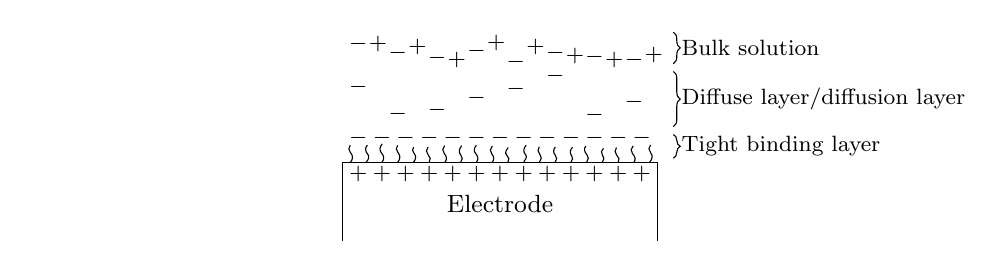
\begin{tikzpicture}
            \small
            \draw (-2,-1) -- (-2,0) -- node[below=3mm]{Electrode} (2,0) -- (2,-1);
    
            \footnotesize
            \foreach \x in {-1.8,-1.5,...,2} {
                \node at (\x,-0.15) {$+$};
            }
            %
            \foreach \x in {-1.9,-1.7,...,2} {
                \draw (\x,0)
                    to[out=45,in=-45] ++({0.02*rand},{0.1+0.02*rand})
                    to[out=135,in=-135] ++({0.02*rand},{0.1+0.02*rand})
                ;
            }
            \foreach \x in {-1.8,-1.5,...,2} {
                \node at (\x,0.3) {$-$};
            }
            %
            \foreach \x in {-1.8,-1.3,...,2} {
                \node at (\x,{0.8+0.3*rand}) {$-$};
            }
            %
            \foreach \x in {-1.8,-1.3,...,2} {
                \node at (\x,{1.4+0.15*rand}) {$-$};
            }
            \foreach \x in {-1.55,-1.05,...,2} {
                \node at (\x,{1.4+0.15*rand}) {$+$};
            }
    
            \draw [decorate,decoration={brace,mirror}] (2.2,1.25) -- node[right]{Bulk solution} ++(0,0.4);
            \draw [decorate,decoration={brace,mirror}] (2.2,0.45) -- node[right]{Diffuse layer/diffusion layer} ++(0,0.7);
            \draw [decorate,decoration={brace,mirror}] (2.2,0.05) -- node[right]{Tight binding layer} ++(0,0.3);

            \path (-6,0) -- (6,0);
        \end{tikzpicture}
        \caption{Electrochemical double layer.}
        \label{fig:echem2layer}
    \end{figure}
    \begin{itemize}
        \item Charge transfer to the analyte occurs through this double layer.
    \end{itemize}
    \item Cyclic voltammetry.
    \begin{itemize}
        \item One of the most common experiments in electrochem.
        \item You sweep between two potentials linearly, plotting the current that flows vs. the potential applied.
        \item The anode oxidizes and the cathode gets reduced during the course of the reaction.
        \item A \emph{reversible} electrochemical reaction appears at a certain potential as a "duck."
        \begin{itemize}
            \item Here, the maximum current ($I_{P_c}$; the peak of the duck) and minimum current ($I_{P_a}$; the belly of the duck) should have the same magnitude.
        \end{itemize}
        \item An \emph{irreversible} electrochemical reaction appears at a certain potential as a one-sided hump or dip.
        \item As stated last time, the peak-to-peak separation should be about \SI{59}{\milli\volt}, but it almost never is.
        \begin{itemize}
            \item \SI{57}{\milli\volt} or \SI{59}{\milli\volt}??
            \item This is the origin of the following equation (possibly related to the SHE vs. $\pH$ one from \textcite{bib:CHEM26700Notes}?).
            \begin{equation*}
                E_{P_c}-E_{P_a} = \frac{\SI{0.059}{\volt}}{n}
            \end{equation*}
        \end{itemize}
        \item There is also a scan-rate dependence on peak separation given by
        \begin{equation*}
            i_P = \num{2.99e-5}\cdot n(\alpha n)^{1/2}AC_0^*D^{1/2}V^{1/2}
        \end{equation*}
        \begin{itemize}
            \item $n$ is the number of electrons.
            \item $\alpha$ is the transfer coefficient.
            \item $A$ is the area of the electrode.
            \item $C_0^*$ is the concentration.
            \item $D$ is the diffusion coefficient.
            \item $V$ is the sweep voltage.
        \end{itemize}
    \end{itemize}
    \item Differential pulse voltammetry.
    \begin{itemize}
        \item This is another technique that allows better resolution than CV for closely spaced features.
        \item More??
    \end{itemize}
    \item Rotating disk or ring electrodes.
    \begin{itemize}
        \item Diffusion is difficult to account for in electrochemistry.
        \item With rotation, we can eliminate diffusion.
        \item We can also add an outside ring around the active electrode to further characterize any compound generated.
        \item If the electrode is rotating, the diffusion path of particles in solution is to move toward the center of the working electrode from underneath and then be spun out to the sides.
    \end{itemize}
    \item Anything else I missed in this lecture??
\end{itemize}




\end{document}